% IMS
% Projekt
% Juraj Holub
% xholub40@stud.fit.vutbr.cz

\documentclass[a4paper, 11pt]{article}
\usepackage[utf8]{inputenc}
\usepackage[czech]{babel}
\usepackage[IL2]{fontenc}
\usepackage{times}
\usepackage[left=1.5cm,top=2.5cm,text={18cm,25cm}]{geometry}
\usepackage[unicode]{hyperref}
\usepackage{amsmath, amsthm, amsfonts, amssymb}
\usepackage{dsfont}
\setlength{\parindent}{1em}
\usepackage{hyperref}
\usepackage{graphicx}
\usepackage{float}
\usepackage{wrapfig}
\usepackage{listings}
\usepackage{url}
\usepackage{cite}
\usepackage{algorithm, algorithmic}
\usepackage{multicol}
\usepackage{color}
%\date{}

\lstset{
	basicstyle=\small\ttfamily,
}

\begin{document}
\begin{titlepage}
	\begin{center}
		\Huge
		\textsc{Fakulta informačních technologií \\
			Vysoké učení technické v~Brně} \\
		\vspace{\stretch{0.382}}
		{\LARGE
			IMS - Modelování a simulace \\ 
			\medskip 
			\Large{
				Ohrev vody v rodinnom dome solárnym systémom.
			}
			\vspace{\stretch{0.618}}}
		\setlength{\parindent}{0.3em}\\
		{\Large 2019} \\
		{\Large Juraj Holub (xholub40)}\\
		{\Large Matej Parobek (xparob00)}
	\end{center}
\end{titlepage}

\tableofcontents
\newpage

\section{Úvod}
Stavebníctvo má v dnešnej dobe veľký dopad na životné prostredie. Spôsob získavania tepelnej energie pre ohrev obytných objektov pomocou alternatívnych zdrojov produkuje nezanedbateľne menšie množstvo CO$_2$ spalín. Táto práca analyzuje systém na ohrev vody pomocou solárneho panelu, ktorý ohrieva zásobník s vodou. Výsledok práce je zhodnoťenie dopadu získavania tepelnej energie zo solárnych panelov na životné prostredie oproti získavaniu tepla spaľovaním zemného plynu a vyhodnotenie efektívnosti navrhovaného systému. 

\subsection{Zdroje infromácií a autori práce}
Postupy a výpočetné vzťahy pre návrh konkrétneho solárneho systému boli použité s odbornej publikácie \cite{Cihelka} určenej projektantom solárnej techniky. Pre validáciu návrhu bola použitý konkrétny navhrhovaný projekt publikovaný v nasledujúcej práci \cite{bc_solar_system}. Referenčný návrh vytvoril vedecký pracovník Energetického ústavu Fakulty strojního inženýrství VUT v Brne Ing. Ján Tuhovčák, Ph.D. ako záverečnú prácu a úspešne ju obhájil s klasifikáciou A. Simulačný model vytvorili Juraj Holub A Matej Parobek na základe týchto informácií. 

\subsection{Validácia navrhovaného modelu}
Výsledky našeho návrhu sú korelované s ročným vyhodnotením z hľadiska energetických nárokov objektu, ktoré poskytuje referenčný návrh. Naše výsledky pre rovnaké časové obdobie sa zhodovali s týmito podkladmi. Z tohto hľadiska bol model vyhodnotený ako validný.

\section{Rozbor navrhovaného systému a použitých technológií}

V rodinnom dome je v prevádzke systém na ohrev vody pomocou zemného plynu s bežným kotlom. Denná spotreba teplej vody je približne 50 l na osobu. V rodinnom dome zo 4 obyvateľmi sa spotreba tepla na ohrev vody pohybuje okolo 3 700 kWh za rok. Spotreba je rovnomerná po celý rok, nezávislo od ročného obdobia. Naopak produkcia tepelnej energie pomocou solárnych panelov je závislá na ročnom období. Pre daný solárny panel a rodinný dom miestom v Brne je produkcia tepla pre jednotlivé kalendárne mesiace závislá od nasledujúcich faktorov:
\begin{itemize}
	\item Počet dní v mesiaci.
	\item Objem zásobníka na vodu.
	\item Sklon solárnych panelov, ich plocha a orientácia (juh).
	\item Teoreticky dopadajúca slnečná energia (príloha \ref{tabulky}, obrázok \ref{str34}).
	\item Pomerná dĺžka slnečného svitu (príloha \ref{tabulky}, obrázok \ref{str41}).
	\item Stredná teplota vzduchu (príloha \ref{tabulky}, obrázok \ref{str50}).
	\item Stredná intenzita slnečného žiarenia (príloha \ref{tabulky}, obrázok \ref{str51}).
\end{itemize}

Ak solárna energia v danom mesiaci nepostačuje na pokrytie spotrebovaného tepla tak sa požadovaná energia získava sekundárnym zdrojom, ktorým je plynový kotol. Na druhej strane, prebitky solárnej energie sa v navrhovanom systéme vôbec nevyužívajú. Navrhovaný solárny systém neprodukuje žiadne spaliny CO$_2$. Naproti tomu, spaľovanie plynu produkuje 202g CO$_2$ spalín \footnote{Zdroj \href{https://www.oplyne.info/ecology/porovnanie-produkcie-znecistujucich-latok-so2-tzl-nox-co-a-sklenikoveho-plynu-co2-vyprodukovanych-spalinami-v-rodinnom-dome-vykurovanie-drevom-ciernym-hnedym-uhlim-a-zemnym-plynom/}{https://www.oplyne.info/ecology/porovnanie-produkcie-znecistujucich-latok...}}  na 1 kWh vyprodukovaného tepla. Podľa referenčnej práce sú emisie spojené s vybudovaním solárneho systému porovnateľné s emisiami na vybudovanie pôvodného systému. S tohto dôvodu emisie spojené s vybudovaním systému táto práca neuvažuje. 

\subsection{Postup požitý pre vytvorenie modelu}

Zo získaných vstupných informácií bol vytvorený abstraktný model (IMS\cite{ims_slides} slide 9.). Pre popis časového priebehu bol použitý abstraktný model vo forme Petriho siete (IMS\cite{ims_slides} slide 123.). Pre popis produkcie a spotreby tepelnej energie bol vytvorený abstraktný model vo forme algebraických rovníc. K výslednému abstraktnému modelu bol vytvorený ekvivalentný simulačný model (IMS\cite{ims_slides} slide 44.) v programovacom jazyku C++ za použitia knihovny \textbf{SIMLIB}\footnote{Project SIMLIB: \href{http://www.fit.vutbr.cz/~peringer/SIMLIB/.cs}{http://www.fit.vutbr.cz/~peringer/SIMLIB/.cs}} . Knihovna bola zvolená s ohľadom na zložitoť modelu. Použitie robustnejšej knihovny by vzhľadom na náročnosť abstraktného modelu bolo neprimerané. Táto knihovna poskytuje základné prostriedky pre diskrétne modelovanie (IMS\cite{ims_slides} slide 44.) ako sú procesy (IMS\cite{ims_slides} slide 121.) alebo obslužné linky (IMS\cite{ims_slides} slide 138.) a to pomocou prostriedkov Objektovo Orientovaného Programovania (OOP).

\subsection{Povod použitých technológií}
Na vytvorenie Petriho sieťe boli využité postupy preberané na predmete IMS\cite{ims_slides} v kapitole \textit{Diskrétní simulace}. Použité algebraické vzťahy boli prevzaté s nasledujúcej knihy\cite{Cihelka}. Simulačný model bol implementovaný v jazyku C++ za použitia OOP abstrakcie a funkcionality zo štandardnej knihovny pre štandard z roku 2014. Program je prekladaný pomocou GNU C++ prekladača \texttt{g++} \footnote{GNU project \href{https://gcc.gnu.org/}{https://gcc.gnu.org/}} . Knihovnu SIMLIB  je využívaná pod licenciou GNU LGLP \footnote{GNU Lesser General Public License \href{https://www.gnu.org/licenses/lgpl-3.0.html}{https://www.gnu.org/licenses/lgpl-3.0.html}} . 

\section{Konceptuálny model}
Na základe rozboru navrhovaného systému bol vytvorený konceptuálny model (IMS\cite{ims_slides} slide 48.) popísaný v tejto kapitole.  Najmenšia časová jednotka v modeli je jeden deň. Takáto jednotka bola zvolená preto, že vyprodukované teplo a zároveň jeho spotreba v systéme je počítaná na základe tabuľkových hodnôt vždy pre časové obdobie jeden deň. Pre zmysluplné zhodnotenie výstupov musí model simulovať čas minimálne v rádoch rokov. V opačnom prípade by samotná výstavba alternatívneho zdroja energie vyprodukovala väčšiu záťaž na životné prostredie ako úspora získaná jeho používaním. 


\subsection{Schéma navrhovaného systému} \label{petri_net_section}
Časť konceptuálneho modelu, ktorá reprezentuje časový priebeh modelu pomocou Petriho siete je priložená na obrázku \ref{obr_petri_net}. Stav (IMS\cite{ims_slides} slide 123.) \textit{Nový mesiac} má na začiatku jedenu značku. Táto značka okamžite prechádza do prechodu \textit{mesačné výpočty}, kde prebiehajú algebraické výpočty relevantné pre aktuálny mesiac, ktoré sú popísané ďalej v tejto sekcii. Značka sa presne za mesiac vracia do stavu \textit{nový mesiac} a výpočet prebieha pre ďalší kalendárny mesiac. Prechod z \textit{mesačné výpočty} taktiež vygeneruje množstvo značiek rovné počtu dní aktuálneho mesiaca. Tieto značky postupne (t.j. každý deň v mesiaci) vykonajú prechod \textit{denné výpočty}. V tomto prechode prebiehajú algebraické výpočty relevantné pre aktuálny kalendárny deň.

\begin{figure}[H] 
	\centering
	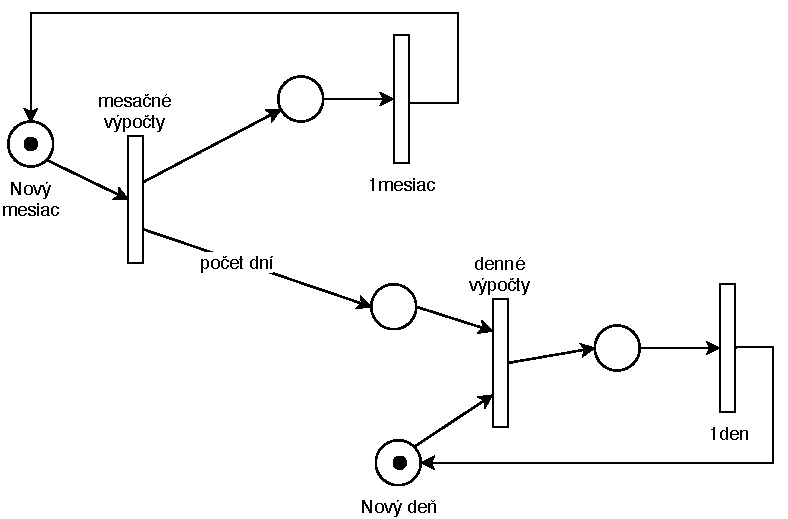
\includegraphics[width=.6\paperwidth]{images/petri_net.pdf}
	\caption{Časť konceptuálneho modelu vo forme Petriho siete, reprezentujúca časový priebeh modelu.}
\end{figure} \label{obr_petri_net}

V prechode \textit{mesačné výpočty} prebiehajú výpočty pre ktoré sú dostupné tabuľkové hodnoty relevantné vždy pre obdobie jedného mesiaca. Pre výpočet účinnosti kolektoru  $Q_{den\ ucinnost}$v danom mesiaci sa použije vzťah \ref{eq:den_ucinnost}. Priepustnosť slnečného žiarenia $\alpha=0.85$ až $0.95$ (\cite{bc_solar_system}, str. 21). Plocha solárneho panelu $S_{panel}$ je v $m^2$, sklon strechy (t.j panelu) $t_{sklon}$ je v stupňoch, stredná teplota v dobe slnečného svitu $t_{str}$ (príloha \ref{tabulky}, obr. \ref{str50}) je v $^{\circ}$C a stredná intenzita slnečného žiarenia $I_{str}$ (príloha \ref{tabulky}, obr. \ref{str51}) je jednotkách $Wm^{-2}$.
\begin{equation}\label{eq:den_ucinnost}
Q_{den\ ucinnost} = \alpha - S_{panel} . \frac{t_{sklon} - t_{str}}{I_{str}}
\end{equation}
Následne sa vypočíta skutočná dopadajúca energia na panel vzťahom \ref{eq:skut_dopad}. Pomerná doba slnečného svitu $\tau_s$ je koeficient platný pre mesto Brno. Teoreticky možná energia dopadajúca za deň na plochu $Q_{den\ teor}$ (príloha \ref{tabulky}, obr. \ref{str34}) je tabuľová hodnota v jednotkách $kWhm^{-2}$.
\begin{equation}\label{eq:skut_dopad}
Q_{skut\ dopad} = \tau_s . Q_{den\ teor}
\end{equation}
Z dopadajúcej energie sa vypočita reálna energia zachytená solárnym kolektorom pomocou vzťahu \ref{eq:skut_zachyt}.
\begin{equation}\label{eq:skut_zachyt}
Q_{skut\ zachyt} = Q_{skut\ dopad} . Q_{den\ ucinnost} . S_{panel}
\end{equation}

Následne sa v prechode \textit{denné výpočty} získa množstvo požadované tepla pre aktuálny deň pomocou vzťahu \ref{eq:spotreba}. Merná tepelná kapacita vody $c_{H_2O}=4180$ je v jednotkách $Jkg^{-1}K^{-1}$. Uvažovaná hustota vody je $\rho_{H_2O} = 995.6kgm^{-3}$ (pri strednej teplote $30^{\circ}C$). Objem zásobníka $V_z$ je v jednotkách litrov. Výstupná teplota vody je $t_2 = 50^{\circ}C$ a vstupná teplota vody je $t_1 = 10^{\circ}C$. Výsledná spotreba v $kWh$ je vynásobená koeficiento $\beta = 1.1$, ktorý uvažuje $10\%$ straty.
\begin{equation}\label{eq:spotreba}
Q_{spotreba} = c_{H_2O} . \rho_{H_2O} . V_z . (t_2 - t_1) . \beta
\end{equation}
Vypočítaná spotreba na deň sa môže pre každý deň mierne líšiť lebo ľudia nespotrebovávajú teplú vodu deterministicky presne. Avšak z dlhodobého hľadiska bude spotreba vody veľmi podobná. Na základe pozorovania spotreby vody v mojej domácnosti, bolo vypozorované že denná spotreba vody sa líši v približnom rozmdzí 10\%. Na základe tohto sa na výpočet skutočnej spotreby použilo normálne rozloženie (IMS\cite{ims_slides} slide 93.) zo strednout hodnotou $\sigma=Q_{spotreba}$ a rozptylom $\mu=0.1*Q_{spotreba}$.

Na záver sa pre aktuálny deň vyhodnotí bilancia vyprodukovanej energie $Q_{skut\ zachyt}$ a požadovanej energie $Q_{spotreba}$ . Spôsob vyhodnotenia je zachytený v algoritme \ref{al:daily_calc}. Výsledkom dennej produkcie tepla môže byť nedostatok solárnej energie (nutnosť použiť plynový kotol) alebo dostatok energie (prípadne jej prebytok).

\begin{algorithm}[H]\label{al:daily_calc}
	\begin{algorithmic}
		\STATE\textbf{Input:} $requiredHeat$
		\STATE\textbf{Input:} $productDaily$
		\STATE$cosumptionDaily \gets \textbf{Normal}(requiredHeat, 0.1 * requiredHeat)$
		\IF {$productDaily < cosumptionDaily$} 
		\STATE $solarDaily \gets productDaily$
		\STATE $fosilDaily \gets cosumptionDaily$
		\ELSE
		\STATE $solarDaily \gets cosumptionDaily$
		\STATE $wasteDaily \gets productDaily - cosumptionDaily$
		\ENDIF 
		\STATE\textbf{Output:} $fosilDaily$
		\STATE\textbf{Output:} $solarDaily$
		\STATE\textbf{Output:} $wasteDaily$
	\end{algorithmic}
	\caption{Daily energetic bilancion.}
\end{algorithm}



\section{Architektúra programu}

Priebeh simulácie je veľmi závislý od simulačného času a to špecificky od mesiaca, ktorý je aktuálne simulovaný. Architektúra programu preto implementuje špeciálnu datovú štruktúru ktorá uchováva informácie o aktuálnom mesiaci v simulačnom čase. Na základe časovej aktuálnej časovej značky sa vyberajú tabuľkové hodnoty popísané v predošlej kapitole.

\subsection{Ročný cyklus}
Ako popisuje sekcia \ref{petri_net_section}, miesto \textit{Nový mesiac} je obsadené 1 procesom vždy na začiatku nového kalendárneho mesiaca. Toto chovanie zabezpečuje proces, ktorý sa vždy uspí na mesiac. Avšak jednotlivé mesiace v roku sa líšia počtom dní. Preto je v rámci celého programu dostupná datová štruktúra, ktorá uchováva aktuálne prebiehajúci mesiac roku, pričom na začiatku je iniciovaná prvým mesiacom každého kalendárneho roku. Pri vstupe do miesta \textit{Nový mesiac}, tento proces vždy nastavený ďalší kalendárny mesiac v roku. Toto chovanie sa cyklicky opakuje po uplinutí roku. Táto štruktúra obsahuje pre každý mesiac príslušný počet dní. .

\subsection{Riadiace procesy}\label{solar_energy_proces}
Riadenie programu je cyklicky predávané na začiatku mesiaca procesu, ktorý po vypočítaní aktuálnych hodnôt predá riadenia postupne každý deň jednému procesu. Proces mesiaca sa teda vždy uspí na počet dní príslušný aktuálnemu mesiacu a zároveň vygeneruje príslušné množstvo procesov na denné výpočty.

\subsection{Tabuľkové hodnoty}
Pre výpočet algebraických rovníc popísaných vpredošlej kapitole sa využívajú tabuľkové hodnoty, ktoré sú implementované v nasledujúcich statických triedach:
\begin{itemize}
	\item \textbf{MeanIntensityOfSunlightBrno}: Trieda obsahuje koštanty reprezentujúce strednú intenzitu slnečného žiarenia v jednotlivých mesiacoch pre Brno. Voľba hodnoty závisí od mesiaca a sklonu strechy. Pre prístup, k tímto hodnotám sa využíva jednoduché rozhranie \textit{get(mesiac, uhol)}, ktoré mapuje \textit{mesiac} a \textit{uhol} na príslušnú hodnotu.
	\item \textbf{TeoreticalIncidentSunlightBrno}: Trieda reprezentuje tabuľkové hodnoty teoretickej možnej energie dopadajúcej za deň na plochu $1m^{2}$ v jednotlivých mesiacoch pre Brno. Voľba hodnoty opäť závisí od mesiaca a sklonu strechy, preto je rozranie rovnaké ako bolo popísané v predošlom bode.
	\item \textbf{SunlightBrno}: Trieda obsahuje tabuľky pre pomernú doba slnečného svitu a taktiež pre strednú teplotu v dobe slnečného svitu v jednotlivých mesiacoch v Brne. Tieto hodnoty sú závislé len od mesiaca, preto je rozhranie tvorené metódov \textit{getMeanTemperature(mesiac)} a \textit{getRatio(mesiac)}.
\end{itemize}

\subsection{Používanie programu}
Vstupom programu sú nasledujúce parametre systému:
\begin{itemize}
	\item \textbf{Čas}: Simuláčný čas programu vždy začína v čase 0 a jeho dĺžku môže uživateľ nastaviť v rokoch.
	\item \textbf{Zásobník}: Objem zásobníka na ohrev teplej vody v litroch. Všeobecne sa doporučuje voliť v násobkoch 50 litrov, čo je priemerná hodnota spotreby na jednu osobu za deň.
	\item \textbf{Plocha kolektorov}: Plocha zachytávajúca slnečné svetlo v $m^2$.
	\item \textbf{Sklon kolektorov}: Sklon strechy je rovný sklonu kolektorov. Je možné simulovať len pre nasledujúce uhly: $0^{\circ}, 15^{\circ}, 30^{\circ}, 45^{\circ}, 60^{\circ}, 75^{\circ}, 90^{\circ}$.
\end{itemize}

Program sa dá preložiť spustením priloženého \texttt{Makefile} a následne spustiť:\\
\texttt{./ims-project -years 1 -tank 200 -area 6 -degree 30} \\
Výstupom programu sú nasledujúce informácie:
\begin{itemize}
	\item Celková spotrebovaná solárna energia v $kWh$ za odsimulované časové obdobie.
	\item Celková spotrebovaná fosilná energia v $kWh$ za odsimulované časové obdobie.
	\item Vyprodukovaná prebytočná (nevyužitá) solárna energia v $kWh$ za odsimulované časové obdobie.
	\item Celkovo spotrebovaná energia v $kWh$ za odsimulované časové obdobie.
	\item Vyprodukované emisie $CO_2$ v $kg$, zo solárnym systémom.
	\item Vyprodukované emisie $CO_2$ v $kg$, bez solárneho systému.
\end{itemize}

\section{Simulačné experimenty}
V tejto sekcii sa na základe výsledkov simulačných experimentov zhodnotí dopad produkcie tepelnej energie zo solárnych panel na životné prostredie v porovnaní s energiou získanou spaľovaním zemného plynu. Na vytvorený model sa aplikovalo niekoľko experimentov s cieľom zistiť efektívnosť systému pre rôzne vstupné parametre.

\subsection{Experiment 1}
Pre overenie validity naimplementovaného modelu bol odsimulovaný experiment s rovnakými vstupnými parametrami ako systém navrhovaný v referenčnej práci\cite{bc_solar_system}:

\begin{table}[H]
	\centering
	\begin{tabular}{|c|c|}
		\hline
		Čas {[}rok{]} & 1 \\ \hline
		Zásobník {[}liter{]} & 200 \\ \hline
		Plocha kolektorov {[}m$^2${]} & 6 \\ \hline
		Sklon kolektorov {[}$^{\circ}${]} & 30 \\ \hline
	\end{tabular}
	\caption{Vstupné parametre systému pre experiment 1.}
	\label{tab:exp1_input}
\end{table}
Energetická bilancia referenčného návrhu\cite{bc_solar_system} a výsledky simulácie sú zobrazené v tabuľke \ref{tab:exp1_output}. Z tabuľky vyplíva, že výsledky simulácie sú veľmi podobné referenčnému návrhu. S tohto hľadiska bol model vyhodnotený ako validný. Navrhovaný systém povedie až k 70\% poklesu produkcie CO$_2$ emisií. Až 42\% solárnej energie vyprodukovanej tímto systémom bude tvoriť prebytok a nebude využitá.

\begin{table}[H]
	\centering
	\begin{tabular}{|c|c|c|}
		\hline
		& Experimentálne výsledky & Referenčné výsledky \\ \hline
		Ročná spotreba energie {[}kWh{]} & 3722.64 & 3713.079 \\ \hline
		Solárna energia {[}kWh{]} & 2565.89 & 2547.703 \\ \hline
		Fosilná energia {[}kWh{]} & 1156.75 & 1165.376 \\ \hline
		Nevyužitá solárna energia {[}\%{]} & 42 & - \\ \hline
		CO$_2$ emiie bez solárneho systému {[}kg/rok{]} & 7444.38 & - \\ \hline
		CO$_2$ emisie zo solárnym systémom {[}kg/rok{]} & 2138.00 & - \\ \hline
		Pokles CO2 emisií{[}\%{]} & 70 & - \\ \hline
	\end{tabular}
	\caption{Porovnanie referenčných výsledkov s výsledkami získanými zo simulácie pre rovnaké vstupné parametre.}
	\label{tab:exp1_output}
\end{table}

\subsection{Experiment 2}
V tomto experimente sa uvažoval sklon strechy vždy $30^{\circ}$. Simulovalo sa po obdobie 1 rok a zmyslom experimentu bolo nájsť najvhodnejší pomer plochy kolektorov a objemu zásobníka vzhľadom na pokles vyprodukovaných emisií. Taktiež sa vyhodnocovala predimenzovanoť panelu v zmysle produkcie energie, ktorá sa ďalej nevyužíva. Výsledky experimentu su zobrazené v tabuľke \ref{tab:exp2}. Z výsledkov vyplíva, že zásobník o objeme 150$l$ s panelom o ploche 6$m^2$ znižuje produkciu emisií približne o 75\% ale zároveň až 52\% vyprodukovanej solárnej energie sa nevyužije. Na druhej strane zásobník o objeme 250$l$ s panelom o ploche 3$m^2$ znižuje produkciu emisií približne o 50\% a zároveň len 2\% vyprodukovanej solárnej energie sa nevyužije.

\begin{table}[H]
	\centering
	\resizebox{\textwidth}{!}{%
		\begin{tabular}{|c|c|c|c|c|c|c|c|c|c|}
			\hline
			\textbf{\begin{tabular}[c]{@{}c@{}}Plocha\\ panelov\\ {[}m$^2${]}\end{tabular}} & \textbf{\begin{tabular}[c]{@{}c@{}}Objem\\ zásobníka\\ {[}l{]}\end{tabular}} & \textbf{\begin{tabular}[c]{@{}c@{}}Spotreba\\ solárnej\\ energie\\ {[}kWh/rok{]}\end{tabular}} & \textbf{\begin{tabular}[c]{@{}c@{}}Spotreba\\ fosilnej\\ energie\\ {[}kWh/rok{]}\end{tabular}} & \textbf{\begin{tabular}[c]{@{}c@{}}Nevyužitá\\ solárna\\ energia\\ {[}kWh/rok{]}\end{tabular}} & \textbf{\begin{tabular}[c]{@{}c@{}}Nevyužitá\\ solárna\\ energia\\ {[}\%{]}\end{tabular}} & \textbf{\begin{tabular}[c]{@{}c@{}}Spotrebovaná\\ energie\\ celkovo\\ {[}kWh/rok{]}\end{tabular}} & \textbf{\begin{tabular}[c]{@{}c@{}}CO2 emiie \\ bez solárneho\\ systému\\ {[}kg/rok{]}\end{tabular}} & \textbf{\begin{tabular}[c]{@{}c@{}}CO2 emisie \\ zo solárnym\\ systémom\\ {[}kg/rok{]}\end{tabular}} & \textbf{\begin{tabular}[c]{@{}c@{}}Pokles CO2\\ emisií\\ {[}\%{]}\end{tabular}} \\ \hline
			6 & 150 & 2067.54 & 709.26 & 2268.76 () & 52 & 2776.80 & 5609.14 & 1432.71 & 75 \\ \hline
			6 & 200 & 2618.30 & 1093.19 & 1838.57 & 41 & 3711.49 & 7497.21 & 2208.24 & 71 \\ \hline
			6 & 250 & 2998.74 & 1655.82 & 1193.34 & 28 & 4654.56 & 9402.22 & 3344.76 & 65 \\ \hline
			5 & 250 & 3027.34 & 1564.84 & 1078.08 & 26 & 4592.19 & 9276.22 & 3160.98 & 66 \\ \hline
			4 & 250 & 2827.86 & 1838.01 & 546.18 & 16 & 4665.87 & 9425.06 & 3712.78 & 61 \\ \hline
			3 & 250 & 2302.78 & 2341.42 & 48.72 & 2 & 4644.20 & 9381.29 & 4729.67 & 50 \\ \hline
		\end{tabular}%
	}
	\caption{Výsledky experimentu 2 pre rôzne vstupné parametre.}
	\label{tab:exp2}
\end{table}

\subsection{Experiment 3}
Experimentovalo sa so sklonom strechy pre panel o ploche 3$m^2$ a zásobník o objmeme 250$l$ po časové obdobie 1 rok. Výsledky experimentu sa nachádzajú v tabuľke \ref{tab:exp3}. Z výsledkov vyplíva, že pre sklon strechy 0$^{\circ}$ až 45$^{\circ}$ je výsledná produkcia emisií takmer totožná. Na druhej strane, pre strehu zo sklonom 60$^{\circ}$ a viac je úspora emisií značne menšia a pri sklone 90$^{\circ}$ je pokles emisií len 14$^{\circ}$.
\begin{table}[H]
	\centering
	\resizebox{\textwidth}{!}{%
		\begin{tabular}{|c|c|c|c|c|c|c|c|c|}
			\hline
			\textbf{\begin{tabular}[c]{@{}c@{}}Sklon\\ strechy\\ {[}degree{]}\end{tabular}} & \textbf{\begin{tabular}[c]{@{}c@{}}Spotreba\\ solárnej\\ energie\\ {[}kWh/rok{]}\end{tabular}} & \textbf{\begin{tabular}[c]{@{}c@{}}Spotreba\\ fosilnej\\ energie\\ {[}kWh/rok{]}\end{tabular}} & \textbf{\begin{tabular}[c]{@{}c@{}}Nevyužitá\\ solárna\\ energia\\ {[}kWh/rok{]}\end{tabular}} & \textbf{\begin{tabular}[c]{@{}c@{}}Nevyužitá\\ solárna\\ energia\\ {[}\%{]}\end{tabular}} & \textbf{\begin{tabular}[c]{@{}c@{}}Spotrebovaná\\ energie\\ celkovo\\ {[}kWh/rok{]}\end{tabular}} & \textbf{\begin{tabular}[c]{@{}c@{}}CO2 emiie \\ bez solárneho\\ systému\\ {[}kg/rok{]}\end{tabular}} & \textbf{\begin{tabular}[c]{@{}c@{}}CO2 emisie \\ zo solárnym\\ systémom\\ {[}kg/rok{]}\end{tabular}} & \textbf{\begin{tabular}[c]{@{}c@{}}Pokles CO2\\ emisií\\ {[}\%{]}\end{tabular}} \\ \hline
			0 & 2323.60 & 2286.58 & 129.92 & 5 & 4610.18 & 9312.56 & 4618.89 & 51 \\ \hline
			15 & 2500.43 & 2157.83 & 152.83 & 5 & 4658.25 & 9409.67 & 4358.81 & 54 \\ \hline
			30 & 2283.44 & 2358.24 & 41.90 & 1 & 4641.68 & 9376.19 & 4763.64 & 50 \\ \hline
			45 & 2319.83 & 2296.38 & 31.81 & 1 & 4616.21 & 9324.74 & 4638.68 & 51 \\ \hline
			60 & 1829.54 & 2833.67 & 0.00 & 0 & 4663.21 & 9419.68 & 5724.01 & 40 \\ \hline
			75 & 1173.70 & 3498.36 & 0.00 & 0 & 4672.07 & 9437.58 & 7066.70 & 26 \\ \hline
			90 & 646.35 & 4010.42 & 0.00 & 0 & 4656.77 & 9406.68 & 8101.05 & 14 \\ \hline
		\end{tabular}%
	}
	\caption{Výsledky experimentu 3 pre rôzne sklony strechy.}
	\label{tab:exp3}
\end{table}

\subsection{Záver experimentov}
Prebehli tri typy experimentov. Prvý experiment slúžil na overenie validity simulačného modelu. Výsledok modelu potvrdil validitu modelu, ale taktiež oproti referenčnému návrhu solárneho systému poskytol informácie o produkcii emisií a prebytočnej tvorbe solárnej energie. 

V druhom experimente sa vyskúšalo 6 rôznych kombinácií objemu zásobníku a plochy kolektorov s cieľom nájsť optimálne riešenie. Za optimálne riešenie bol zvolený návrh zo zásobníkom o objeme 250$l$ a zo solárnym panelom o ploche 6$m^2$. Takáto zostava neprodukuje takmer žiadnu prebytočnú solárnu energiu. Vyprodukovaná energia je efektívne využívaná. CO$_2$ emisie v tomto prípade poklesnú o polovicu.

V treťom experimente sa vyskúšalo 7 rôznych sklonov strechy na ktorej bude panel umiestnený. Okrem sklonu sa počítalo s parametrami, ktoré sme zvolili v predošlom experimente za optimálne. Výsledok experimentu je fakt, že panel umiestnený na streche v sklone 0$^{\circ}$ až 45$^{\circ}$ produkuje veľmi podobné solárne zisky. Väčší sklon vedie k značnému poklesu výkonnosti solárneho systému. Záverom experimentu je doporučenie navrhovať sklon panelu v rozmedzí do 45$^{\circ}$. Na voľbe presného sklonu v tomto rozmedzí takmer nezáleží lebo efektívnosť solárneho systému pre takto zvolený uhol je takmer zhodná.

\section{Záver}
{\color{red}Závěrem dokumentace se rozumí zhodnocení simulační studie a zhodnocení experimentů (např. Z výsledků experimentů vyplývá, že ... při předpokladu, že ... Validita modelu byla ověřena ... V rámci projektu vznikl nástroj ..., který vychází z ... a byl implementován v ...).
\begin{itemize}
	\item do závěru se nehodí psát poznámky osobního charakteru (např. práce na projektu mě bavila/nebavila, ...). Technická zpráva není osobní příběh autora.
	\item absolutně nikoho nezajímá, kolik úsilí jste projektu věnovali, důležitá je pouze kvalita zpracování simulátoru/modelu a obsažnost simulační studie (rozhodně ne např.: projekt jsem dělal ... hodin, což je víc než zadání předpokládalo. Program má ... řádků kódu). Pokud zdůrazňujete, že jste práci dělali významně déle než se čekalo, pak tím pouze demonstrujete vlastní neschopnost (to platí zejména v profesním životě).
	\item do závěru se velmi nehodí psát "auto-zhodnocení" kvality práce, to je výhradně na recenzentovi/hodnotiteli (např. v projektu jsem zcela splnil zadání a domnívám se, že můj model je bezchybný a výsledky taktéž). Statisticky častý je pravý opak autorova auto-zhodnocení. Pokud přesto chcete vyzdvihnout kvalitu svého díla (což je dobře), tak vaše výroky musí být naprosto nepopiratelně zdůvodněny a prokázány (např. pomocí jiného referenčního přístupu, matematického důkazu, analýzy, ...).
\end{itemize}
}

\newpage
\bibliographystyle{czechiso}
\bibliography{bib}

\newpage
\appendix

\section{Tabuľkové hodnoty pre návrh solárnej tepelnej techniky}\label{tabulky}

Tabuľkové hodnoty boli získané z knihy pre projektantov solárnych systémov\cite{Cihelka}.

\begin{figure}[H] 
\centering
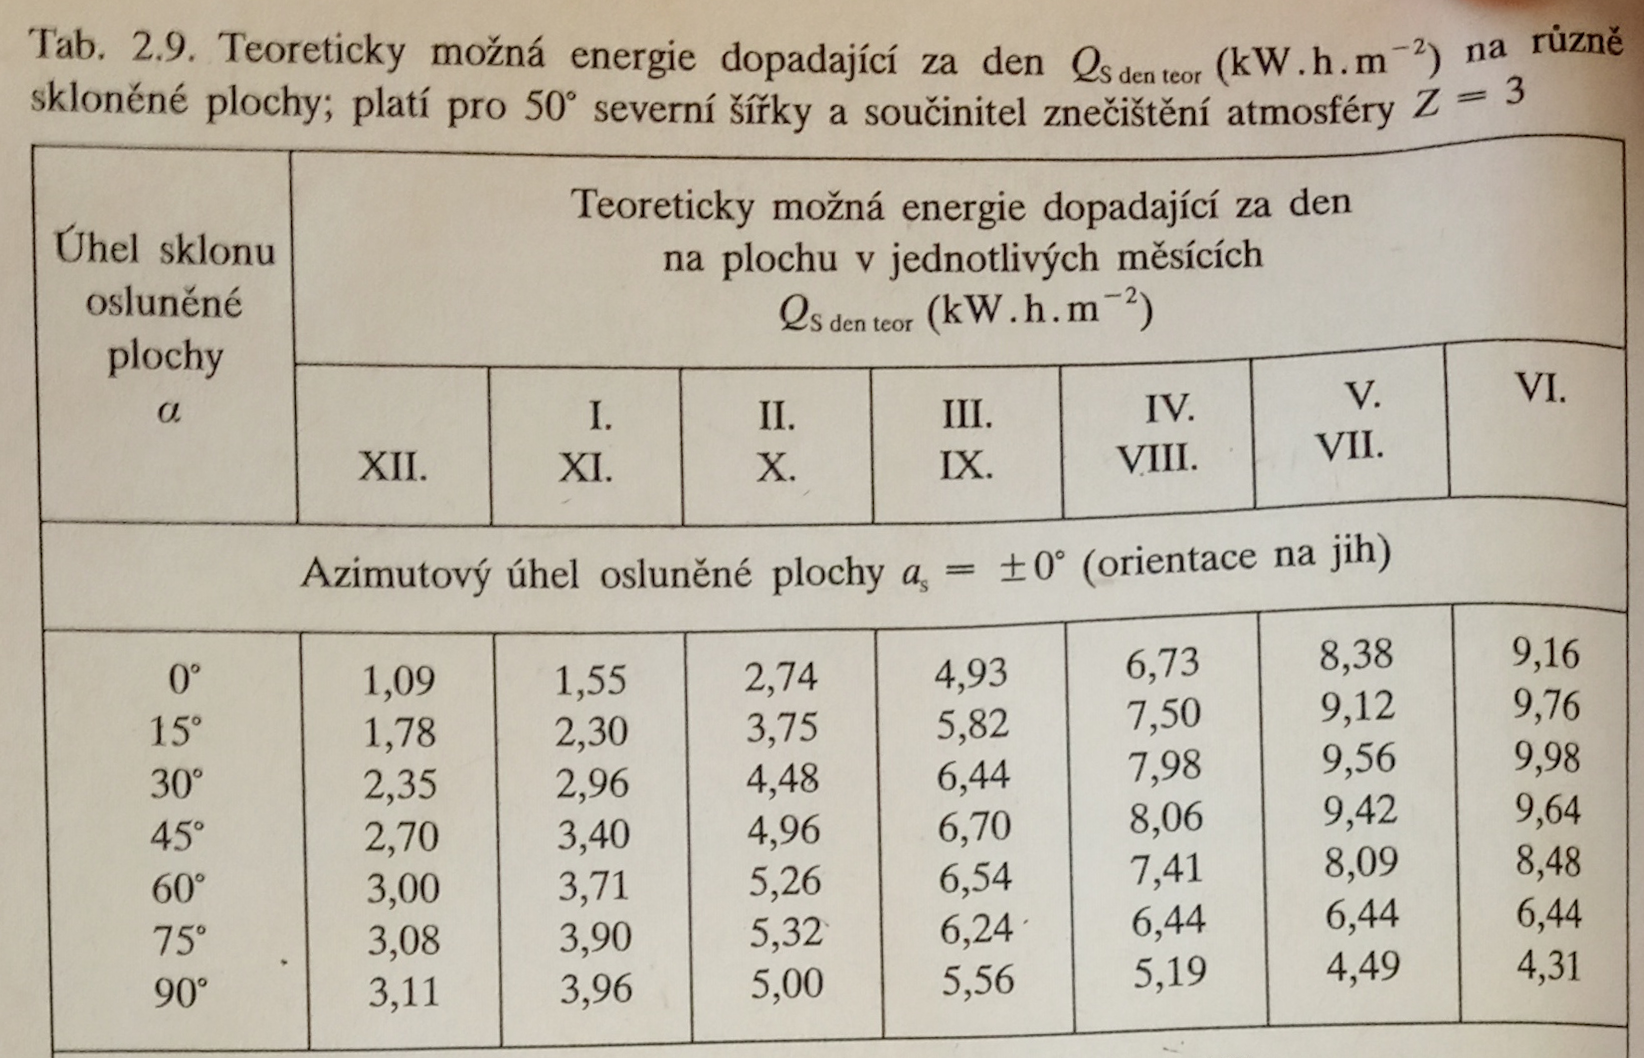
\includegraphics[width=.6\paperwidth]{images/str34.png}
\caption{Teoreticky možná energia dopadajúca za deň na plochu v jednotlivých mesiacoch.}
\label{str34}
\end{figure}

\begin{figure}[H] 
\centering
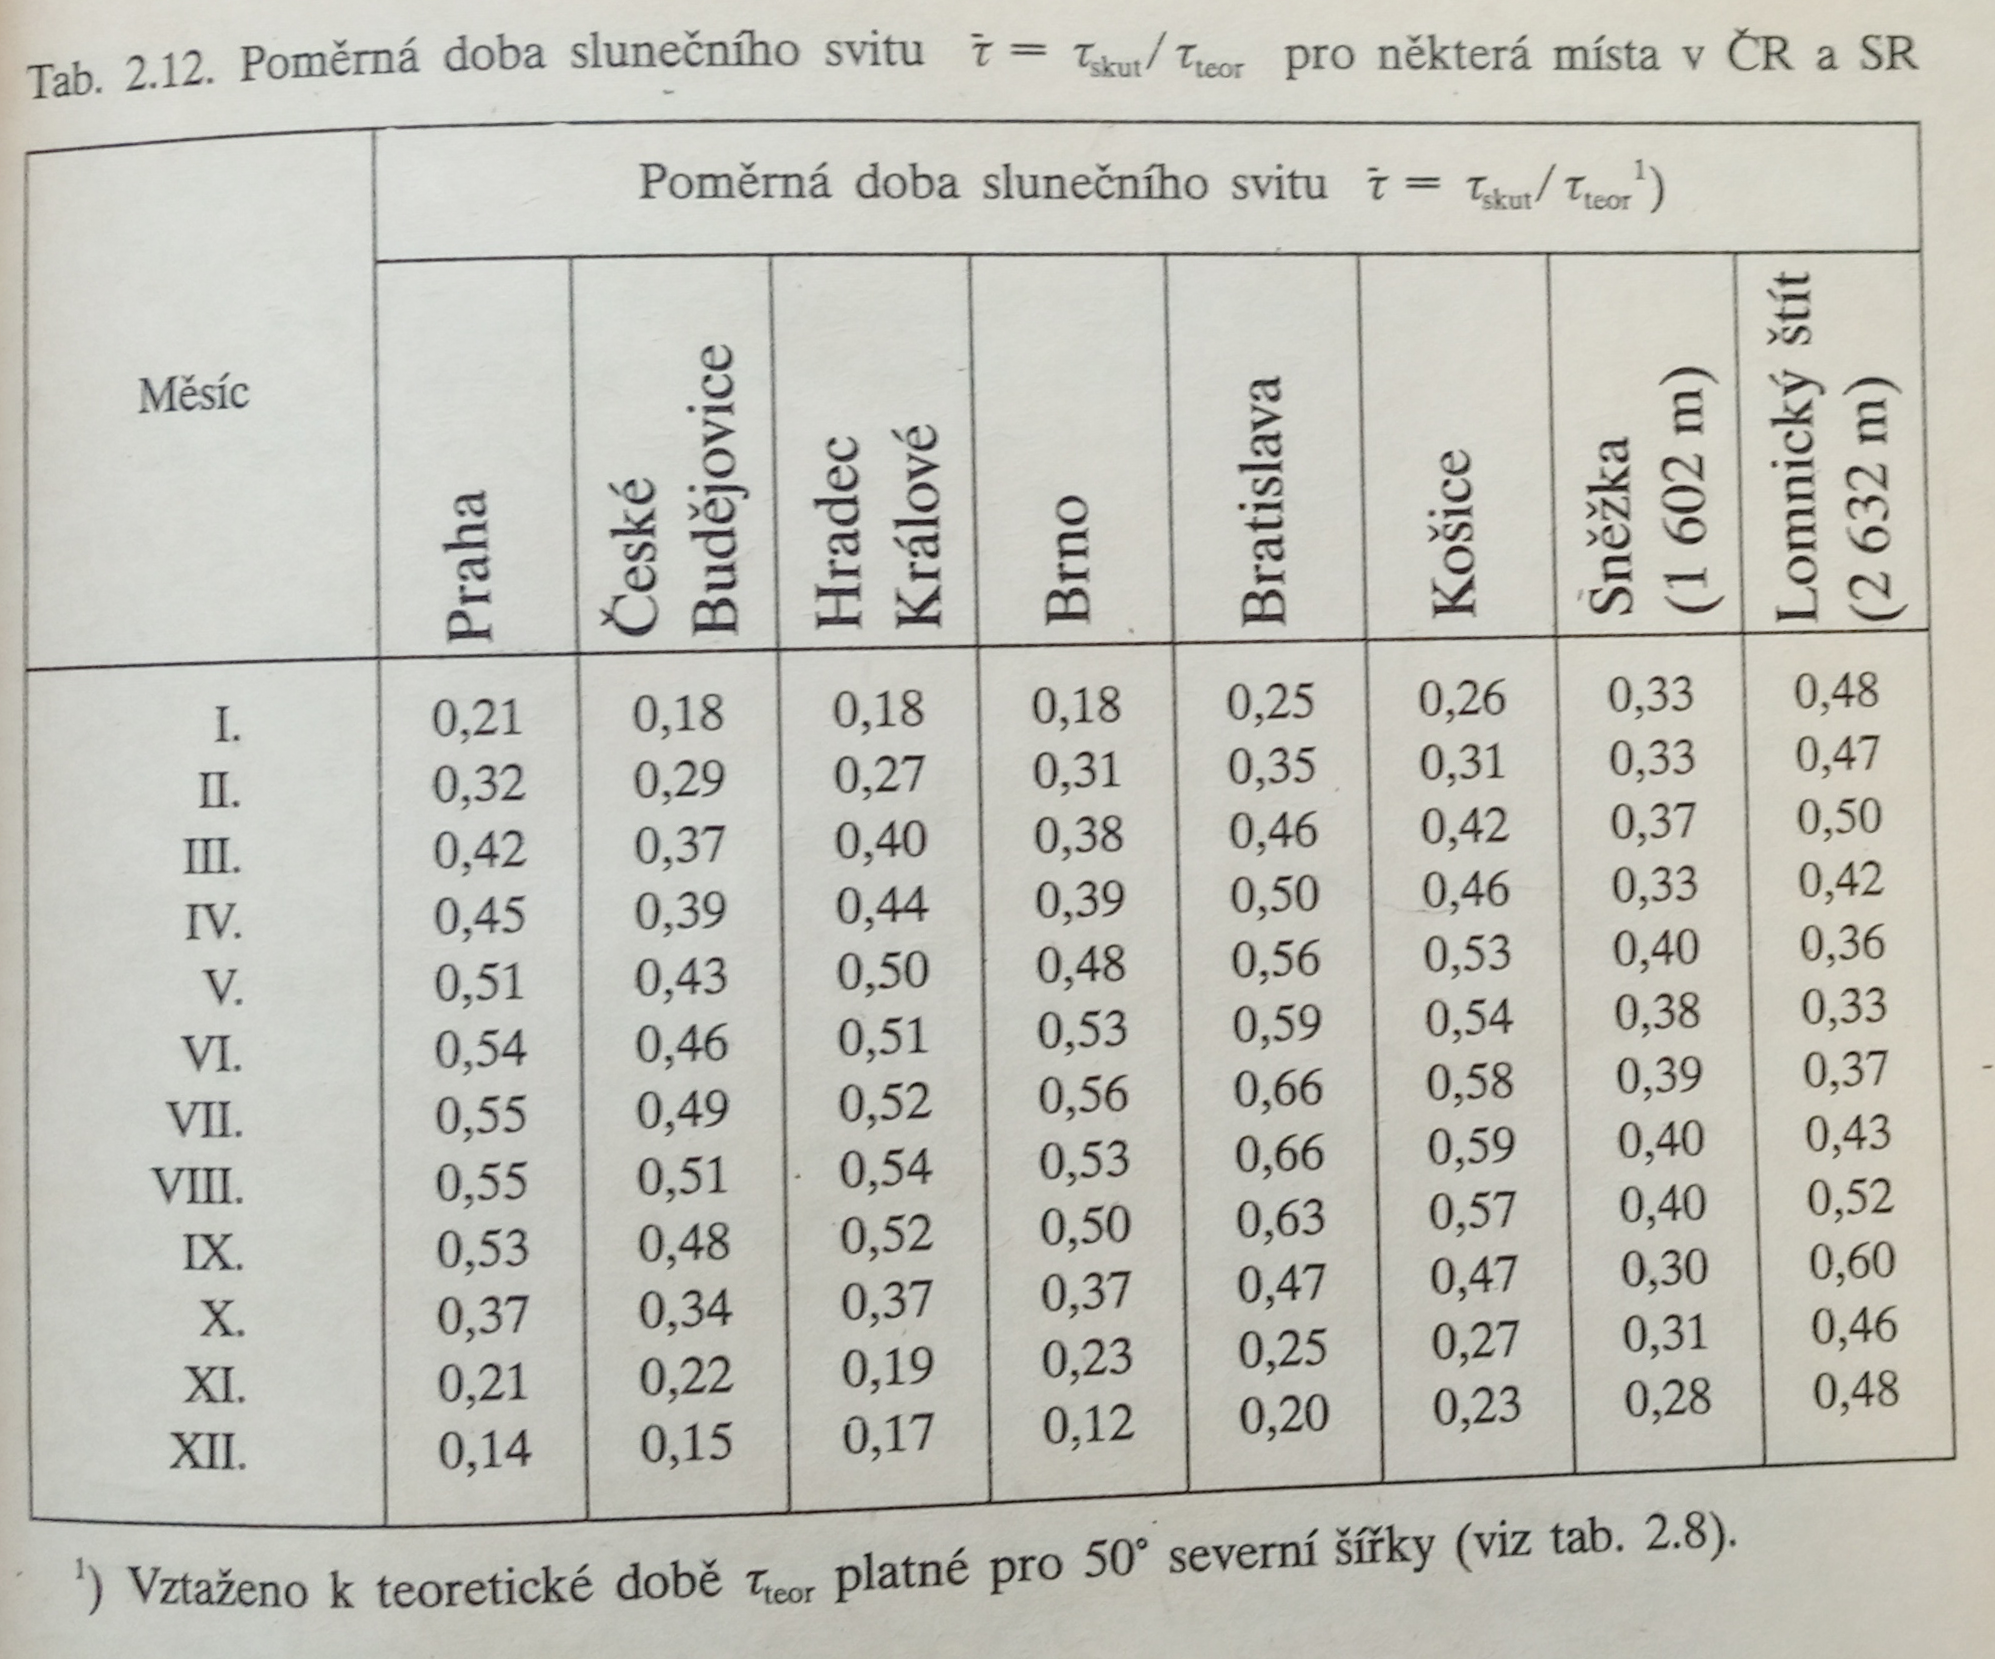
\includegraphics[width=.6\paperwidth]{images/str41.png}
\caption{Pomerná doba slnečného svitu.}
\label{str41}
\end{figure}

\begin{figure}[H] 
\centering
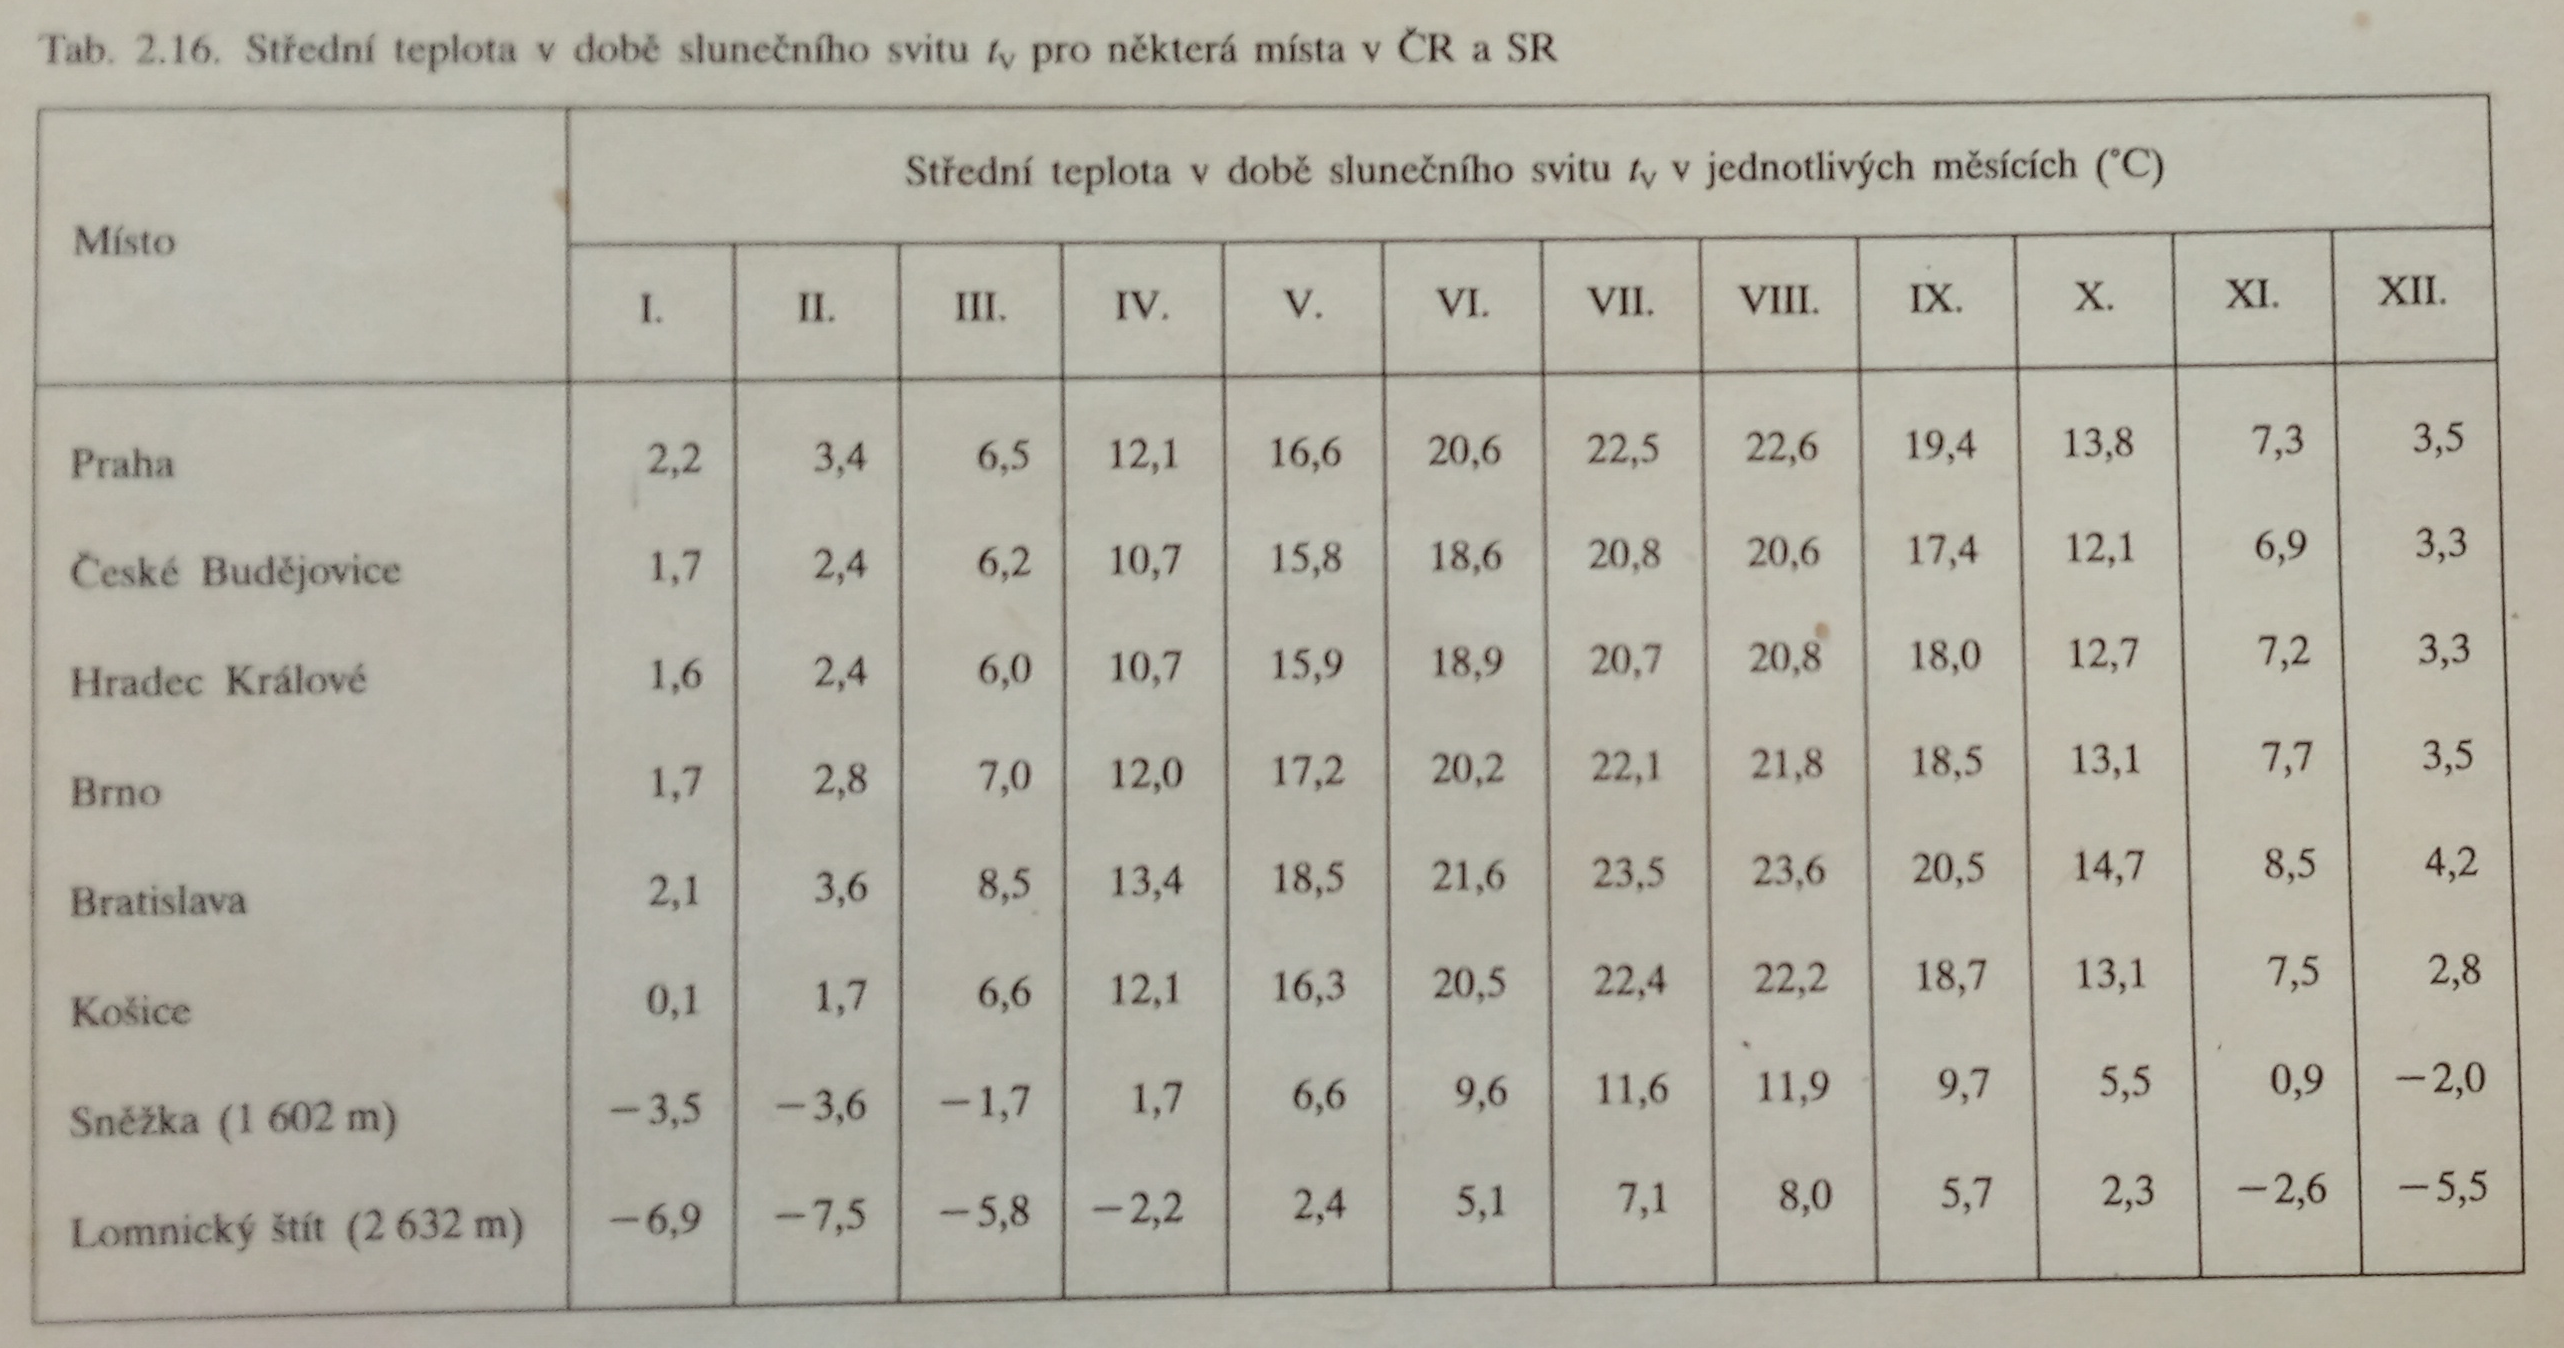
\includegraphics[width=.7\paperwidth]{images/str50.png}
\caption{Stredná teplota v dobe slnečného svitu v jednotlivých mesiacoch.}
\label{str50}
\end{figure}

\begin{figure}[H] 
\centering
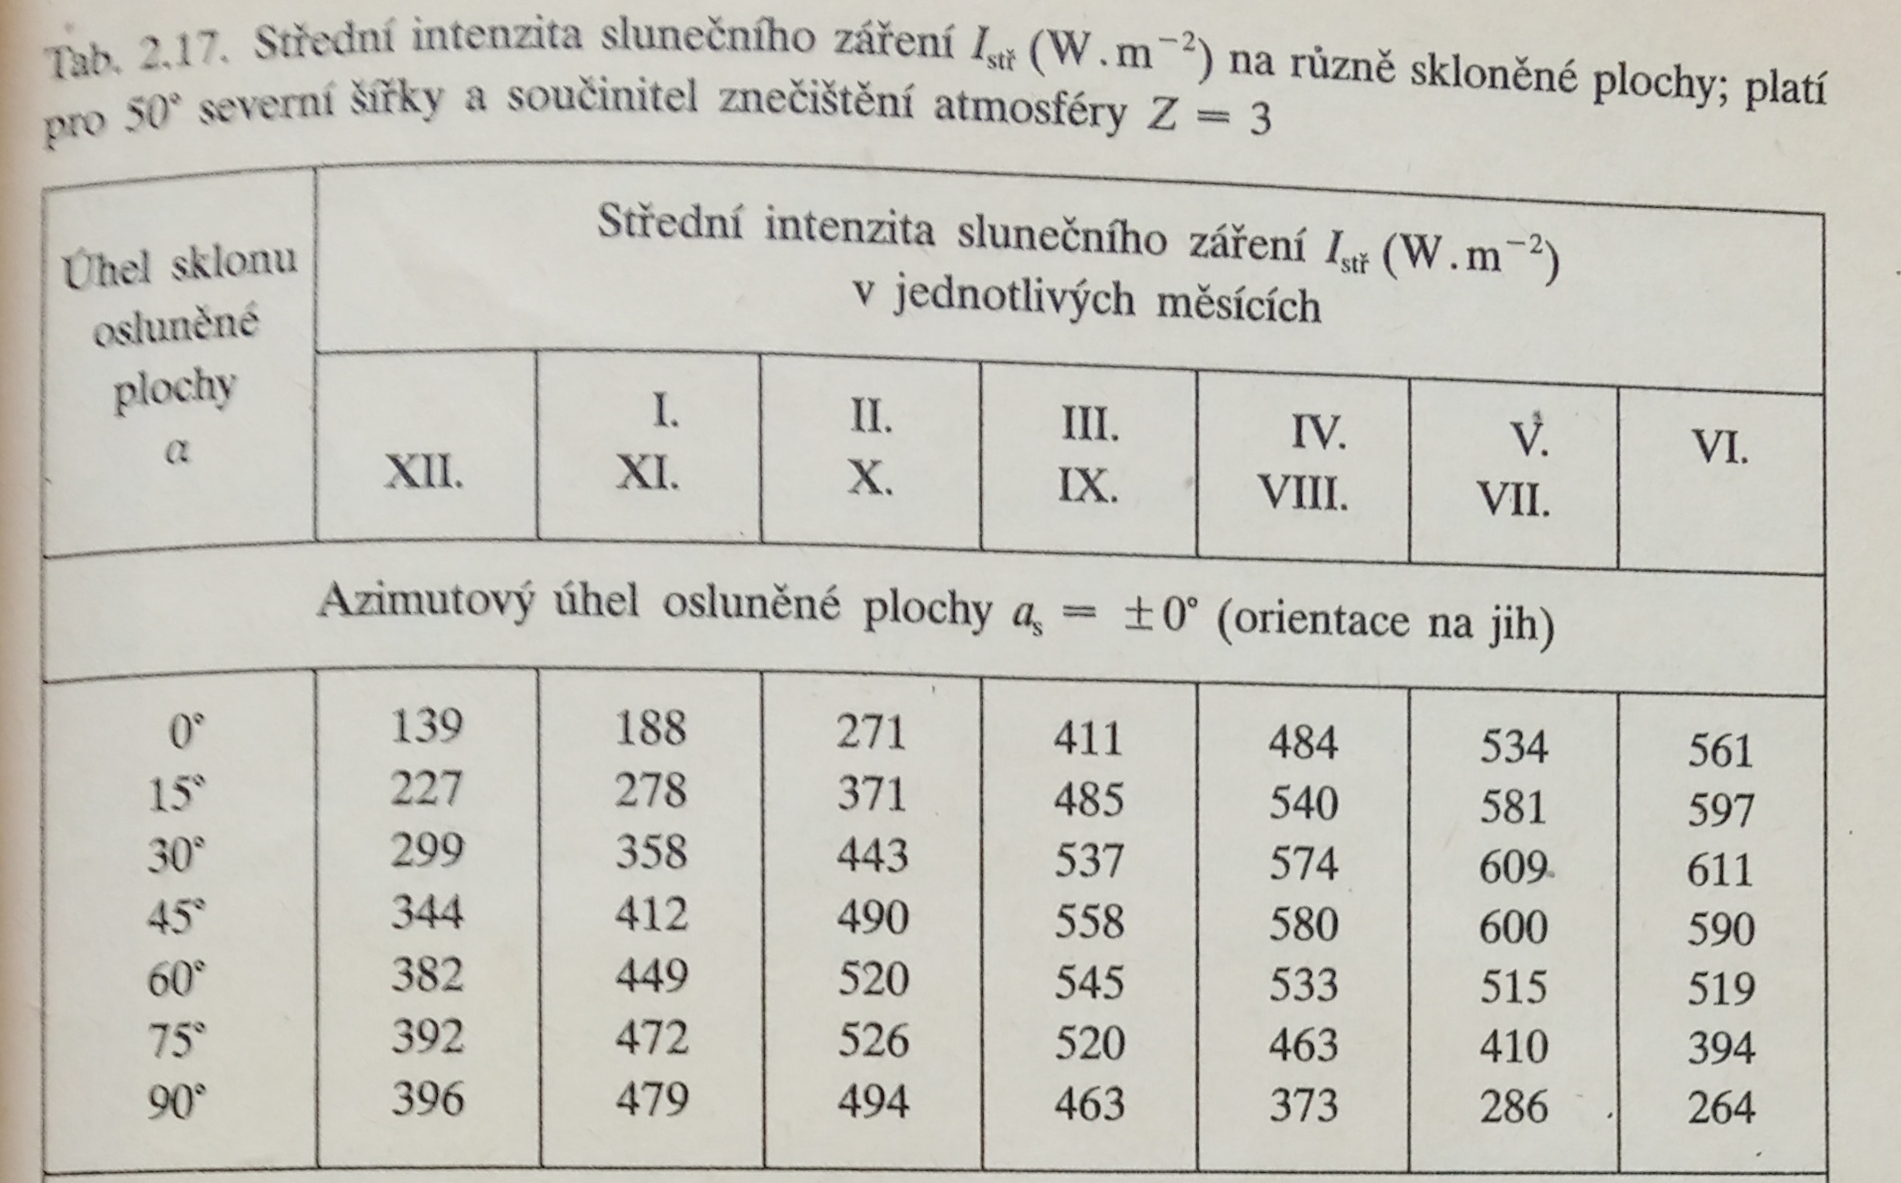
\includegraphics[width=.7\paperwidth]{images/str51.png}
\caption{Stredná intenzita slnečného žiarenia v jednotlivých mesiacoch.}
\label{str51}
\end{figure}


\end{document}
